\documentclass[11pt]{article}
\usepackage[utf8]{inputenc}
\usepackage[T1]{fontenc}
\usepackage{geometry}
\usepackage{graphicx}
\usepackage{amsmath}

\geometry{margin=2.5cm}

\title{Informe de Desempeno\\MPI Document Search Engine}
\author{Proyecto Final}
\date{}

\begin{document}
\maketitle

\section{Resumen}
Este proyecto implementa un motor de busqueda paralelo con MPI basado en
TF-IDF y similitud coseno. En esta version la indexacion se distribuye entre
los procesos (TF-IDF e IDF en paralelo) y se reduce el volumen de datos
transferidos al intercambiar solo el vocabulario global y los Top-K, lo cual
mejora el rendimiento global. El informe presenta el algoritmo, la
paralelizacion y un analisis detallado con las graficas obtenidas.

\section{Conceptos clave (explicados en simple)}
\begin{itemize}
  \item \textbf{Corpus:} conjunto de documentos de texto usados como base de busqueda.
  \item \textbf{Vocabulario:} lista de palabras unicas presentes en el corpus.
  \item \textbf{Tokenizacion:} proceso de dividir el texto en palabras (tokens).
  \item \textbf{TF (Term Frequency):} frecuencia relativa de una palabra en un documento.
  \item \textbf{DF (Document Frequency):} numero de documentos que contienen una palabra.
  \item \textbf{IDF (Inverse Document Frequency):} peso que reduce palabras muy comunes.
  \item \textbf{TF-IDF:} producto TF $\times$ IDF; representa importancia de una palabra.
  \item \textbf{Similitud coseno:} mide el angulo entre dos vectores; 1 significa muy similares.
  \item \textbf{Top-K:} los K documentos con mayor score de similitud.
  \item \textbf{Scatter/Gather/Bcast/Allreduce:} operaciones MPI para repartir,
  recolectar, difundir y reducir datos entre procesos.
  \item \textbf{Rank:} identificador de cada proceso MPI (0 es el master).
\end{itemize}

\section{Generacion de corpus de prueba}
Los corpus usados en las pruebas se generan con \texttt{generate\_corpus.py}.
El script crea un vocabulario sintetico de tamano configurable (por defecto 5000),
genera documentos con una distribucion tipo Zipf (algunas palabras aparecen
mucho mas que otras) y produce una consulta con un numero fijo de terminos.
Esto permite crear conjuntos de 100, 500, 1000 y 5000 documentos de manera
reproducible usando una semilla fija.

\section{Descripcion del algoritmo}
Cada documento se convierte en un vector TF-IDF y la consulta tambien se
convierte en un vector del mismo tamano. Luego se calcula la similitud coseno
entre la consulta y cada documento. Finalmente se ordenan los resultados y se
devuelven los Top-K documentos mas relevantes.

\subsection{TF-IDF}
Para cada termino $t$ en el documento $d$:
\[
  TF(t,d) = \frac{\text{freq}(t,d)}{\text{total de terminos en } d}
\]
\[
  IDF(t) = \log \left(\frac{N}{1 + df(t)}\right)
\]
El vector final es $TF\mbox{-}IDF(t,d)=TF(t,d)\cdot IDF(t)$, donde $N$ es el
numero total de documentos y $df(t)$ es el numero de documentos que contienen
el termino.

\subsection{Similitud coseno}
\[
  sim(q,d) = \frac{q \cdot d}{\|q\|\|d\|}
\]
Los documentos se ordenan de mayor a menor segun esta similitud.

\section{Paralelizacion con MPI}
La version actual distribuye la indexacion y reduce comunicacion:
\begin{enumerate}
  \item \textbf{Particion del corpus:} todos los ranks listan los archivos y
  cargan solo su subconjunto local.
  \item \textbf{Vocabulario global:} cada rank crea un vocabulario local;
  el rank 0 los fusiona y lo difunde con \texttt{MPI\_Bcast}.
  \item \textbf{DF/IDF en paralelo:} cada rank calcula DF local y se combina
  con \texttt{MPI\_Allreduce} para obtener DF global e IDF.
  \item \textbf{TF-IDF local:} cada rank calcula TF-IDF solo para sus documentos.
  \item \textbf{Top-K distribuido:} cada rank calcula similitudes y envia su
  Top-K; el master los fusiona con \texttt{MPI\_Gatherv}.
\end{enumerate}
Este flujo elimina el \texttt{Scatter} de la matriz TF-IDF completa y reduce
el trafico total a vocabulario y Top-K.

\section{Pipeline del \texttt{search\_engine}}
El flujo completo del programa puede resumirse en los siguientes pasos:
\begin{enumerate}
  \item \textbf{Lectura del corpus:} cada rank lista los archivos y carga solo
  su particion local en memoria.
  \item \textbf{Vocabulario global:} se construye un vocabulario local y se
  fusiona en el master para producir el vocabulario global.
  \item \textbf{Calculo de DF/IDF:} cada rank calcula DF local, se reduce para
  obtener DF global y se calcula IDF.
  \item \textbf{Vectorizacion:} cada rank calcula TF-IDF para sus documentos
  y el vector TF-IDF de la consulta.
  \item \textbf{Busqueda:} se calcula la similitud coseno para cada documento
  local y se obtiene el Top-K local.
  \item \textbf{Recoleccion final:} el master recibe los Top-K locales,
  realiza el merge y entrega el ranking final.
\end{enumerate}
Este pipeline esta alineado con la forma en la que se midieron los tiempos
de indexacion, busqueda y merge en los resultados experimentales.

\section{Mejora de rendimiento: TF-IDF/IDF en paralelo y menos datos transferidos}
La ultima mejora se enfoco en reducir el tiempo de indexacion y el trafico MPI.
Antes, el master calculaba el vocabulario, IDF y toda la matriz TF-IDF, y luego
distribuia esa matriz completa con \texttt{MPI\_Scatterv}. Esto generaba dos
problemas: (1) una fase de indexacion totalmente serial en el master y
(2) un volumen grande de datos enviados a todos los procesos.

En la version actual, el trabajo se distribuye desde el inicio:
\begin{itemize}
  \item \textbf{Vocabulario paralelo:} cada rank construye su vocabulario local
  y el master los fusiona para crear el vocabulario global.
  \item \textbf{DF/IDF paralelos:} cada rank calcula DF local y se realiza un
  \texttt{MPI\_Allreduce} para obtener DF global y calcular IDF en todos.
  \item \textbf{TF-IDF local:} cada rank calcula TF-IDF solo para sus documentos,
  eliminando la necesidad de enviar una matriz completa por la red.
  \item \textbf{Comunicacion reducida:} solo se transfieren el vocabulario global
  y los Top-K locales, lo que reduce significativamente el trafico MPI.
\end{itemize}

El impacto se observa en los resultados: el tiempo de \textbf{Scatter} es
practicamente cero (Figura~\ref{fig:breakdown}) y el tiempo total baja con P en
corpus grandes (Figura~\ref{fig:total-time}), con speedup notable hasta 32
procesos (Figura~\ref{fig:speedup}). Con el merge jerarquico, el costo de
recoleccion de Top-K se reduce, aunque sigue siendo el principal limite en
P muy altos.

\section{Mejora de rendimiento: merge jerarquico de Top-K}
Para reducir el costo del \texttt{Gather}, se reemplazo la recoleccion plana
de resultados por un \textbf{merge jerarquico} (reduccion en arbol). En lugar
de enviar todos los Top-K directamente al master, los procesos se emparejan y
fusionan sus listas de manera progresiva:
\begin{itemize}
  \item Cada rank parte con su Top-K local ordenado.
  \item En cada nivel, ranks pares reciben el Top-K de su pareja, fusionan y
  conservan solo los mejores K resultados.
  \item El numero de mensajes se reduce a $\log_2(P)$ niveles y el volumen total
  transferido disminuye, ya que cada fusion mantiene solo K elementos.
\end{itemize}
Este esquema reduce la presion sobre el master y baja el tiempo de merge en
configuraciones con muchos procesos, aunque el overhead de sincronizacion
todavia limita el escalamiento para P muy altos.

\section{Configuracion experimental}
Las pruebas se realizaron en el cluster usando los mismos parametros que el
estudio anterior. Se evaluaron corpus de 100, 500, 1000 y 5000 documentos, con
vocabulario de alrededor de 5000 palabras, Top-K = 10 y multiples repeticiones.
Los resultados se almacenan en \texttt{results/}.

\subsection{Configuracion de ejecucion en el cluster}
La ejecucion en el cluster se definio mediante un script SLURM
\texttt{run\_search.sh} con los siguientes parametros principales:
\begin{itemize}
  \item \textbf{Particion:} \texttt{legacy}
  \item \textbf{Tiempo maximo:} 04:00:00
  \item \textbf{Nodos:} 4
  \item \textbf{Tareas por nodo:} 16 (hasta 64 procesos en total)
  \item \textbf{Memoria por CPU:} 512 MB
  \item \textbf{MPI:} OpenMPI GCC 4.1.6 (modulo \texttt{mpi/openmpi-gcc11/4.1.6})
\end{itemize}
Esta configuracion permite ejecutar los experimentos con P = 1, 2, 4, 8, 16,
32 y 64 procesos, manteniendo coherencia con las pruebas de escalabilidad
reportadas en este informe.

\section{Resultados y analisis}

\subsection{Tiempo total}
La Figura~\ref{fig:total-time} muestra reducciones claras del tiempo total al
aumentar procesos, especialmente para corpus grandes. Por ejemplo, para 5000
documentos el tiempo total baja de 46.1 s (P=1) a 11.5 s (P=4) y alcanza un
minimo de 8.37 s en P=32; en P=64 vuelve a crecer por sobrecarga. En corpus
pequenos el overhead limita la mejora.

\begin{figure}[htbp]
  \centering
  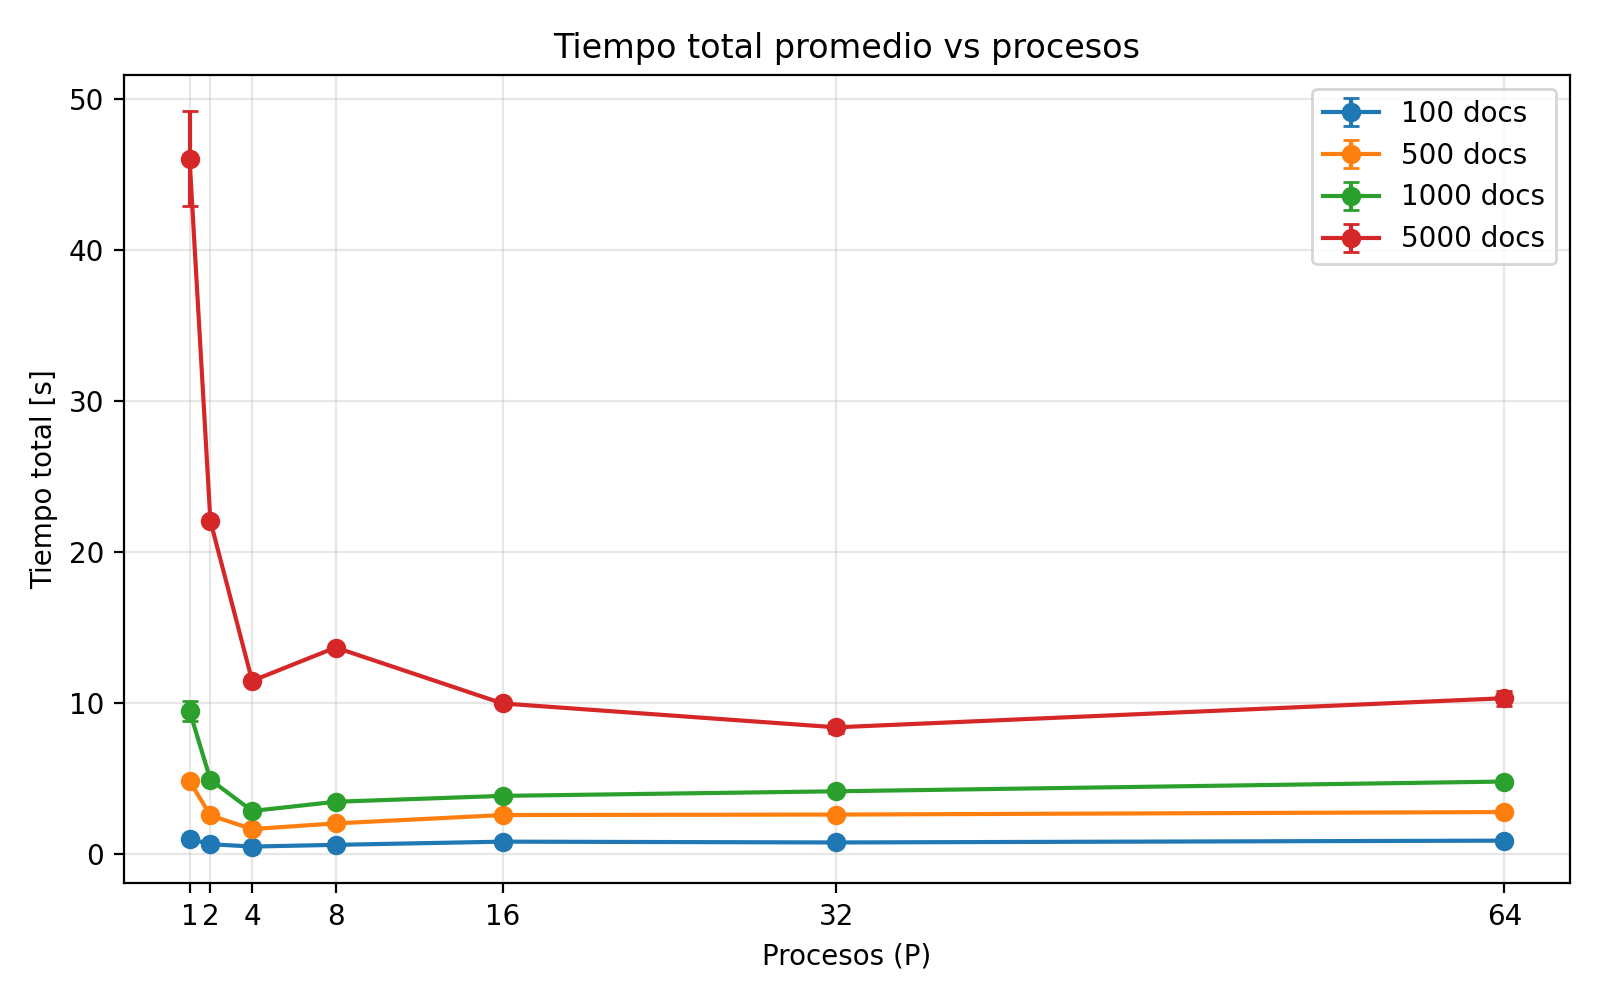
\includegraphics[width=0.9\linewidth]{figuras/total_time_vs_procs.png}
  \caption{Tiempo total promedio vs procesos.}
  \label{fig:total-time}
\end{figure}

\subsection{Speedup y eficiencia}
La Figura~\ref{fig:speedup} evidencia mejoras sustanciales: para 5000 documentos
el speedup llega a 4.02 (P=4) y 5.50 (P=32). Para 1000 documentos el mejor
speedup es 3.35 (P=4). La eficiencia es alta en P=2--4 para corpus grandes
(cercana a 1), pero disminuye al aumentar P por sobrecarga de sincronizacion
y recoleccion de resultados.

\begin{figure}[htbp]
  \centering
  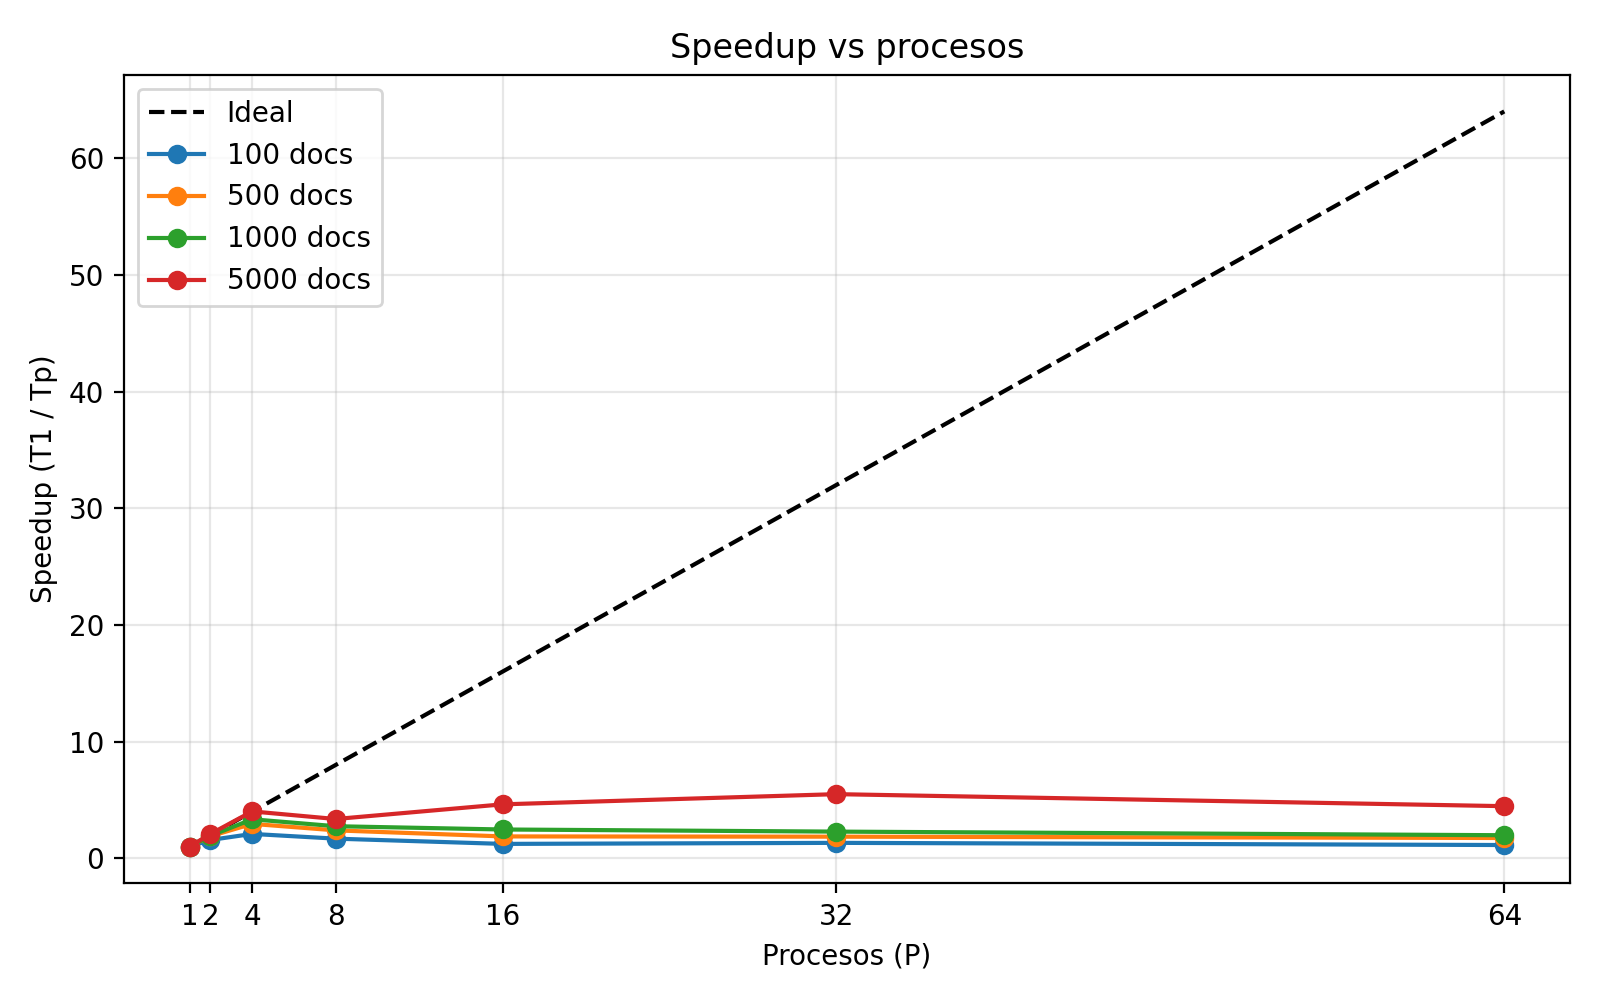
\includegraphics[width=0.9\linewidth]{figuras/speedup_vs_procs.png}
  \caption{Speedup por cantidad de procesos.}
  \label{fig:speedup}
\end{figure}

\begin{figure}[htbp]
  \centering
  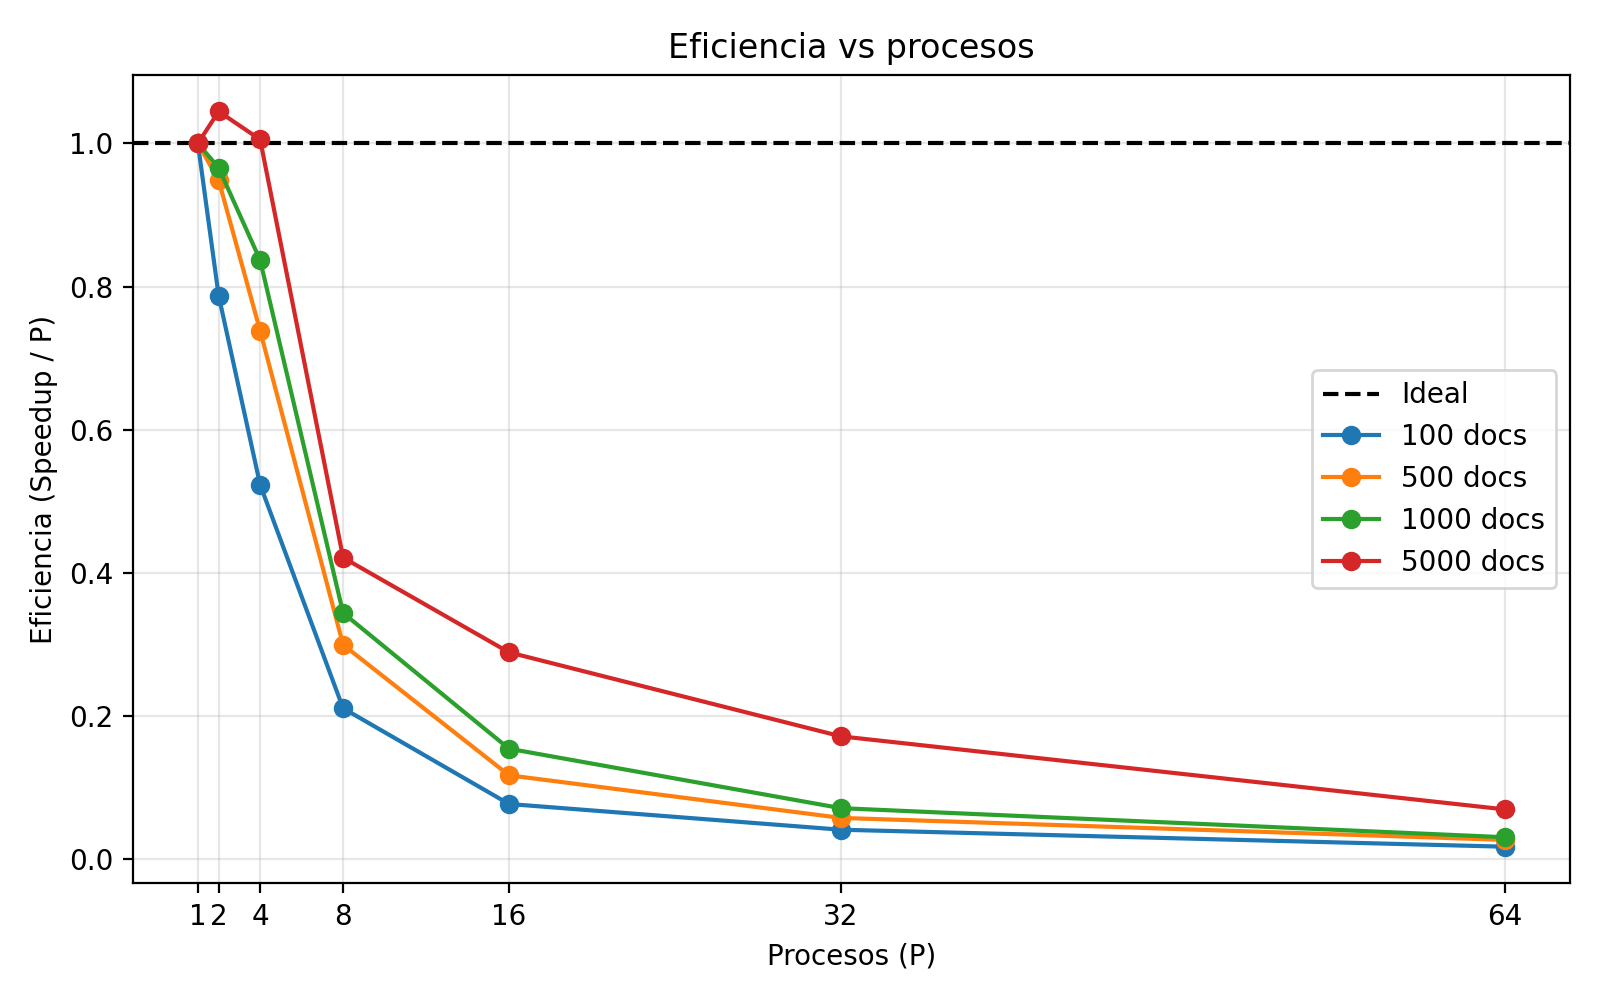
\includegraphics[width=0.9\linewidth]{figuras/efficiency_vs_procs.png}
  \caption{Eficiencia por cantidad de procesos.}
  \label{fig:eff}
\end{figure}

\subsection{Desglose por fases}
La Figura~\ref{fig:breakdown} muestra que \textbf{Scatter} desaparece (tiempo
aproximadamente cero) al eliminar la distribucion de la matriz TF-IDF.
La indexacion ahora se reparte entre procesos y disminuye con P. Con el
merge jerarquico, el costo de \textbf{Gather/Merge} baja en P altos, pero sigue
creciendo con el numero de procesos y domina el overhead en escalas grandes.

\begin{figure}[htbp]
  \centering
  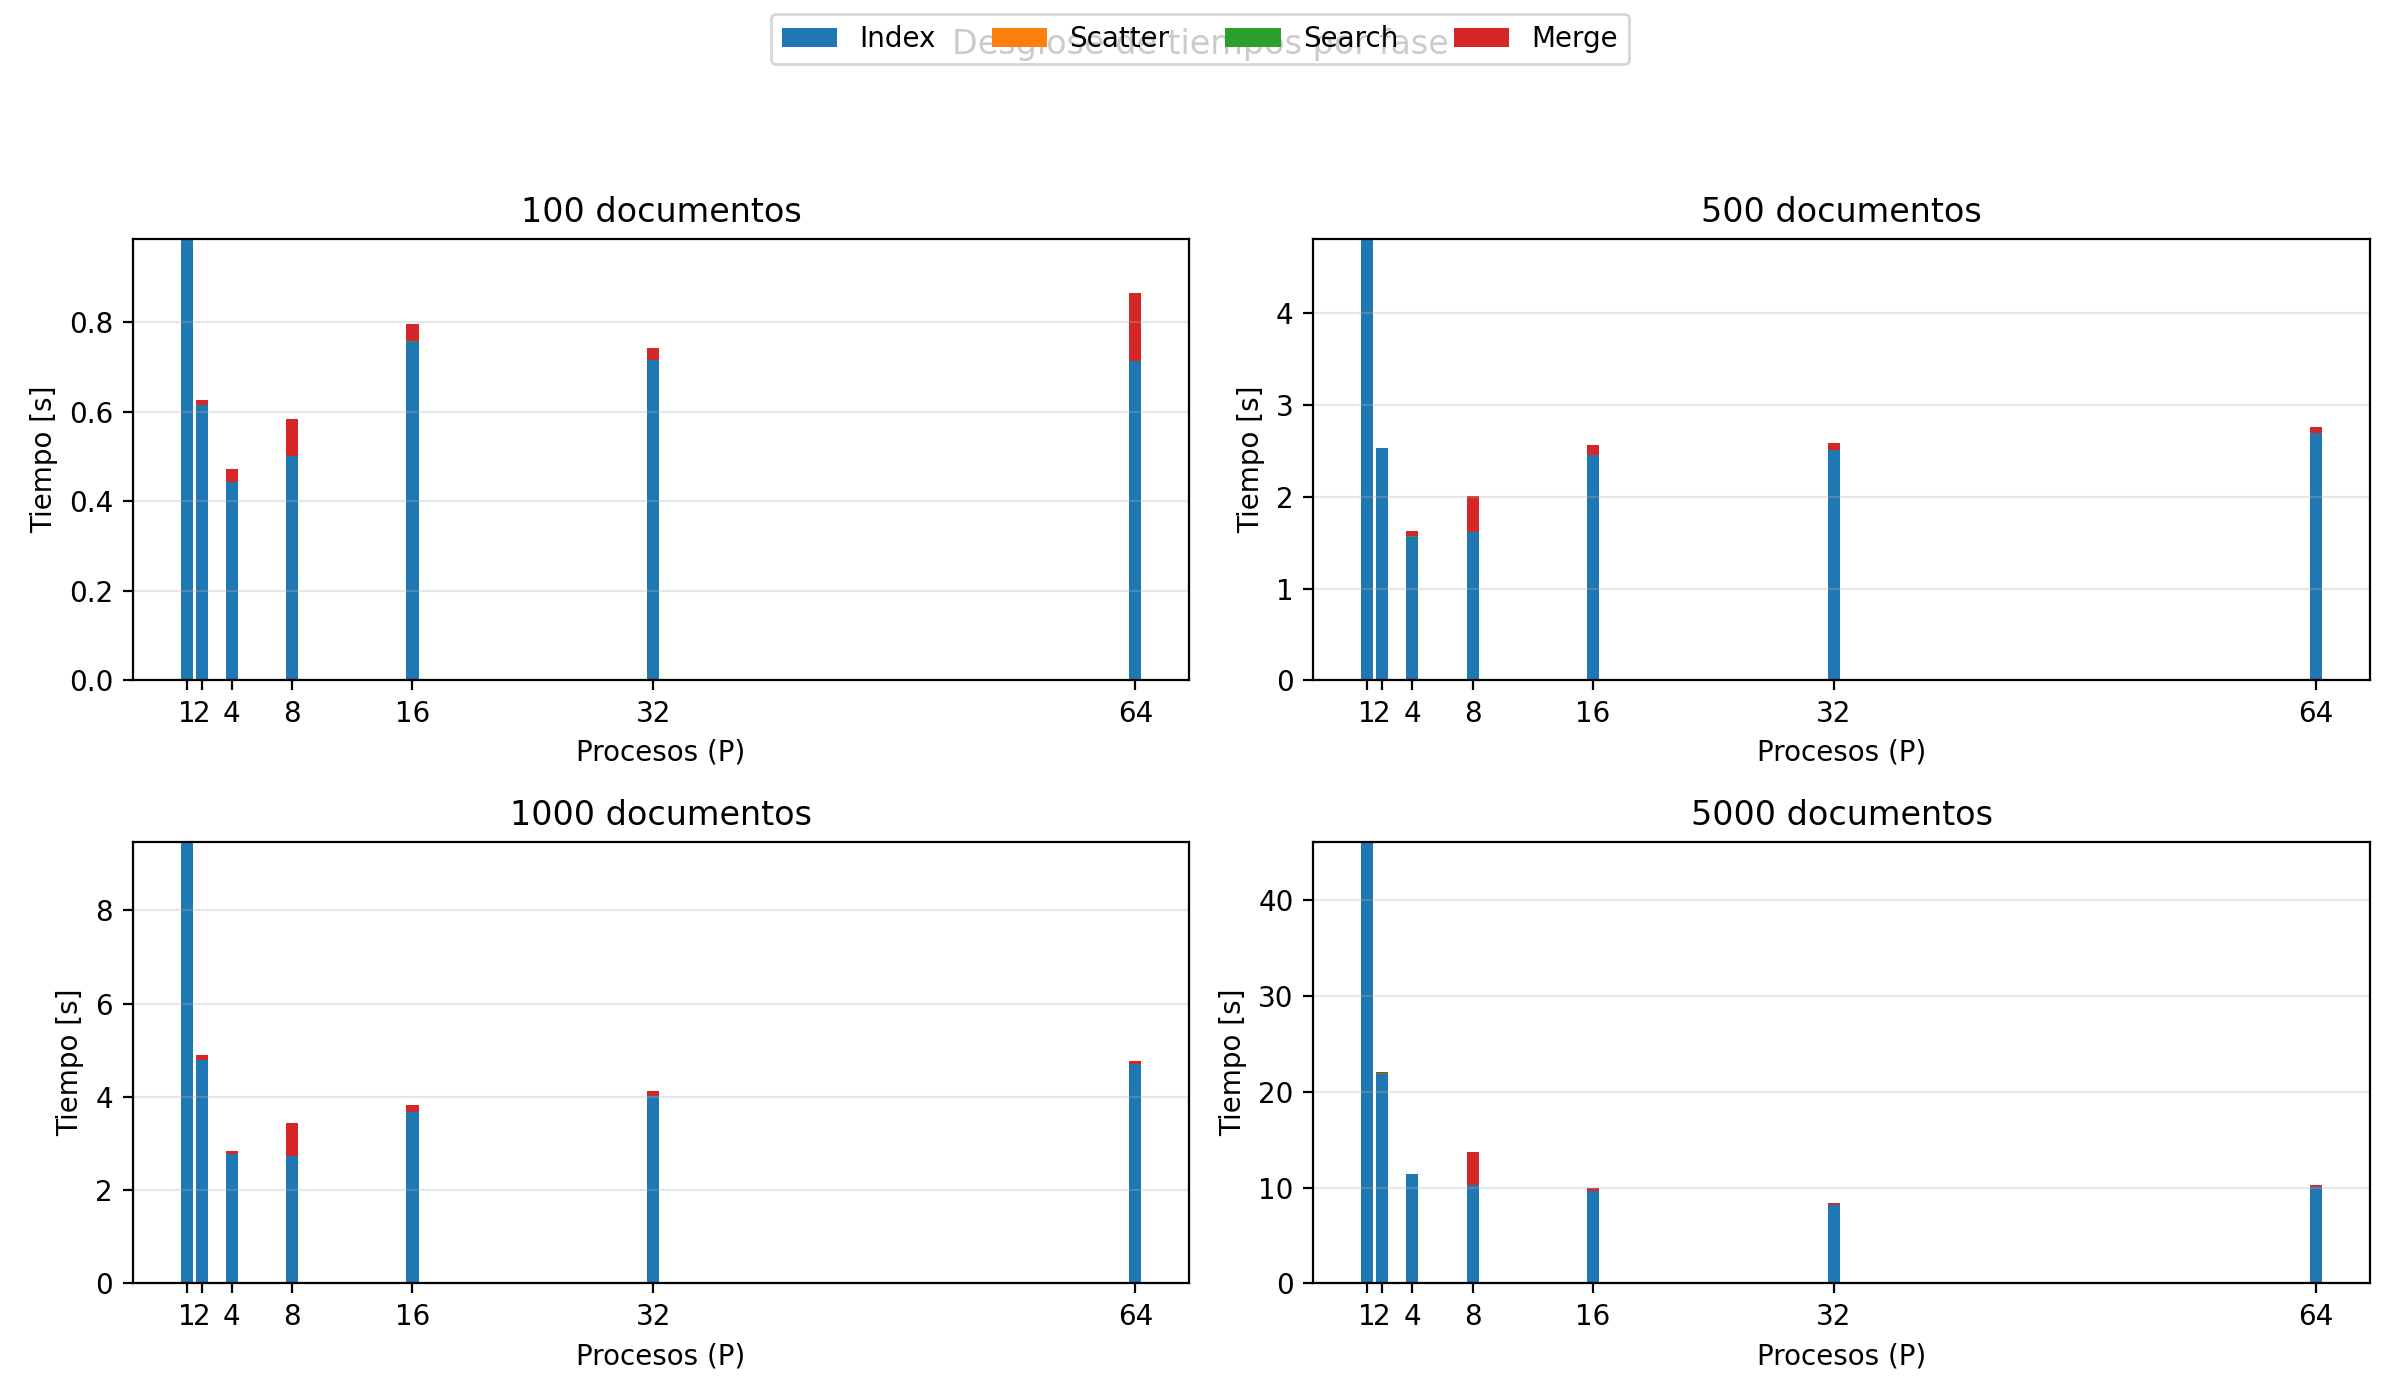
\includegraphics[width=0.95\linewidth]{figuras/time_breakdown_stacked.png}
  \caption{Desglose de tiempos por fase (Index/Scatter/Search/Merge).}
  \label{fig:breakdown}
\end{figure}

\subsection{Observaciones clave}
\begin{itemize}
  \item \textbf{Mejora global:} la indexacion paralela reduce el tiempo total
  de forma notable, especialmente en corpus grandes.
  \item \textbf{Overhead en P altos:} el merge jerarquico reduce el costo del
  \texttt{Gather/Merge}, pero aun limita la eficiencia cuando P es muy grande.
  \item \textbf{Mejor punto operativo:} para 5000 documentos, P=16--32 ofrece
  el mejor balance entre speedup y eficiencia.
\end{itemize}

\section{Conclusiones}
La version paralelizada de TF-IDF e IDF mejora claramente el rendimiento y
reduce el trafico MPI, eliminando el \texttt{Scatter} de matrices grandes.
El merge jerarquico disminuye el costo de recoleccion de Top-K, pero en P muy
altos el overhead de fusion y sincronizacion sigue siendo el principal limite.

\section{Como reproducir las graficas}
Ejecutar los scripts desde la raiz del proyecto:
\begin{verbatim}
python3 plot_scaling.py
python3 plot_breakdown.py
\end{verbatim}
Las figuras se guardan en el directorio \texttt{figuras/}.

\end{document}
